\section{Architecture}

\paragraph{Software Architecture}
What is Software Architecture? \textit{The way different part of the system connect together}. Is based on sub-system and how this sub-system work together

Can be defined as new types of abstraction that capture the essential
properties of major subsystems and how they interact. Software Architecture is the set of fundamental choices that affect the
structure, quality, and efficiency of a software system. This is important
because it affects the system’s scalability, maintainability, and ability to evolve

\begin{definition}\textbf{Webster's dictionary} The art or practice of designing and building structures and especially habitable ones 
\end{definition}

\begin{definition}
A unifying or coherent form or structure
\end{definition}

Why we call Software Architecture "Architecture"? Inherit a lot of ideas and concepts from building architecture. The most important are: \textit{multiple views}; \textit{architectural style}; \textit{styles and materials}

\paragraph{Multiple views}
Building architecture uses multiple views and different stakeholder linked with different natures and accountability.
\begin{itemize}
    \item \textit{Owner}, does not know how, but knows perfectly \textbf{why}
    \item \textit{Architect}, needs to project and formalize something that fit completely with owner’s needs, the \textbf{what}
    \item \textit{Builder}, needs to design \textbf{how} the what will be built
\end{itemize}
For each stakeholder there’s a specific view. How map the idea in Software Architecture? Each developer have a specific view

\paragraph{Architectural style}
The architectural styles has both the list of the design elements and the formal relationships that allow everyone to use the architecture. We can use architecture style both to constrain the architecture and to coordinate operating
architects. Style embodies those decisions that suffer \textit{erosion} and \textit{drift}.
\begin{itemize}
    \item Erosion means that is not completely clear the reasonal between the architecture so the developer use this not in the proper way
    \item Drift means that the architecture was build for a given reason then reason change overtime and the architecture is not able to follow this evolution
\end{itemize}

\paragraph{Styles and materials}
The material aspects of the design elements provide both aesthetic and engineering bases for an architecture. What could be material inside Software Architecture? Frameworks and technologies, the same function can be obtained
using different sub-systems

\paragraph{Project execution pyramid}
\begin{center}
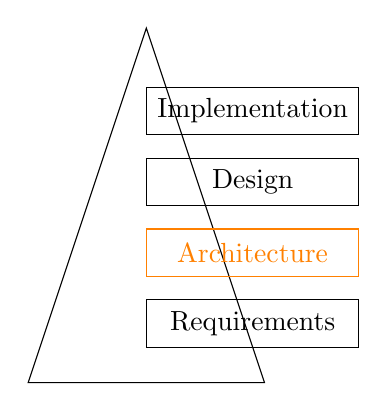
\begin{tikzpicture}[scale=3]
% draw the triangle
\draw (0,0) -- (1.0,0) -- (0.5,1.5) -- cycle;
% draw the rectangles and their labels
\draw (0.5,0.15) rectangle node {Requirements} (1.4,0.35);
\draw[orange] (0.5,0.45) rectangle node {Architecture} (1.4,0.65);
\draw (0.5,0.75) rectangle node {Design} (1.4,0.95);
\draw (0.5,1.05) rectangle node {Implementation} (1.4,1.25);
% add the caption
%\node[above right] at (1.5,1.05) {ciao};
\end{tikzpicture}
\end{center}
It's also described in Perry and Wolf's $1992$ paper, perhaps not as a pyramid shape but as "parts" of the software. We've $4$ layer in the pyramid
    \begin{itemize}
        \item \textit{Requirements}, determination of the information and the characteristics needed by the user of the system
        \item \textit{Architecture}, selection of architectural elements, their interactions and the constraints to satisfy the requirements and serve a basis for the design
        \item \textit{Design}, detailed interfaces of the design elements, algorithms and procedures needed to support the architecture and satisfy the requirements
        \item \textit{Implementation}, representation of the algorithms and data types that satisfy the desing, architecture and requirements
    \end{itemize}

\paragraph{Architecture as a framework for abstractions}
By abstraction we mean identifying a pattern, naming it, defining it, analyzing it and finding a way to invoke it by its name, in order to avoid errors. The basic idea is to omit the right details in the appropriate context, simplifying the interpretation of the result. Example of abstraction are:
\begin{itemize}
    \item \textit{Object Oriented Programming}, abstract data types provide a useful way to organize a software system
    \item \textit{Layered Systems}, OSI layer. System organized hierarchically, with each layer providing service to the layer above it
    \item \textit{Event-oriented programming}, the trigger is the use of this abstraction
\end{itemize}

\paragraph{System-Subsystem Abstraction}
We could use this idea of abstraction to
design system that could be constructed combining subsystem. And this is what an architecture is, a big system that you abstracted combining several subsystem. Each subsystem could be/have an architecture itself and may perform a specific function or a more common function

Identifying and classifying the system functions that are common to many applications is a significant first step to the development of software architecture

%Architecture pillars
\subsection{Architecture pillars}
\begin{enumerate}
    \item \textit{Being the framework for satisfying requirements}, know in advance that all we’re going to build fit completely requirements. Functional, technical and security requirements
    \item \textit{Being the technical basis for design}, modularization and detailed interfaces of the design elements, their algorithms and procedures, and the data types needed to support the architecture and to satisfy the requirements reducing the freedom of the developer
    \item \textit{Being the managerial basis for cost estimation and process management}
    \item \textit{Enabling component reuse}
    \item \textit{Allowing a tidy scalability}, scalability in a people perspective (if I’ve to add some people in the team)
    \item \textit{Avoiding handover and people lock-in}
\end{enumerate}

\begin{definition}
    An architecture is focus on company, mindset, not only technical issue
\end{definition}

%Extra: Foundations for the Study of Software Architecture - Perry, Wolf
\subsection{Extra: Foundations for the Study of Software Architecture - Perry, Wolf}
This paper present a model of software architecture that consists of three components: \textit{elements}, \textit{form}, and \textit{rationale}. Elements are either processing, data, or connecting elements. Form is defined in terms of the properties of, and the relationships among, the elements – that is, the constraints on the elements. The rationale provides the underlying basis for the architecture in terms of the system constraints, which most often derive from the system requirements

\paragraph{Building architecture}
The classical field of architecture provides some of the
more interesting insights for software architecture. While the subject matter for the two is quite different, there are a number of interesting architectural points in building architecture that are suggestive for software architecture: multiple views, architectural styles; style and engineering; style and materials

\paragraph{Context of architecture}
We characterize the different parts of the software
\begin{itemize}
    \item \textit{Requirements}, determination of the information
    \item \textit{Architecture}, selection of architectural elements
    \item \textit{Design}
    \item \textit{Implementation}
\end{itemize}

\paragraph{The model} 
The paper propose the following model of software architecture:
$$\mathit{Software\;Architecture = \{Elements, Form, Rationale\}}$$
In the paper we can distinguish three different classes of architectural elements: processing elements, data elements, connecting elements.

In building architecture, the rationale explicates the underlying philosophical aesthetics that motivate the architect. In software architecture, the rationale instead explicates the satisfaction of the system constraints.

\newpage